\documentclass[review]{elsarticle}
\graphicspath{ {./figures/} }
\usepackage{algorithm}
\usepackage{amsmath}
\usepackage{amssymb}
\usepackage{array}
\usepackage{booktabs}
\usepackage{longtable}
\usepackage{pdflscape}
\usepackage{float}
\usepackage{xcolor}
\usepackage{enumitem}
\usepackage{hyperref}
\setlist{nosep}
\floatstyle{plaintop}
\restylefloat{table}

\journal{Expert Systems with Applications}

\bibliographystyle{model5-names}\biboptions{authoryear}

\begin{document}

\begin{frontmatter}

\begin{titlepage}
\begin{center}
\vspace*{1cm}

\textbf{\large Interpretable-by-Construction Factor Reduction with Interpolative Boolean Algebra for Forecasting Risk and Performance of Financial Index Time Series}

\vspace{1.5cm}

% Author names and affiliations
Aleksa Radosav\v{c}evi\'c$^a$ (ar20235065@student.fon.bg.ac.rs), Ana Poledica$^a$ (ana.poledica@fon.bg.ac.rs), Pavle Milo\v{s}evi\'c$^a$ (pavle.milosevic@fon.bg.ac.rs), Vesna Bogojevi\'c-Arsi\'c$^a$ (vesna.bogojevic.arsic@fon.bg.ac.rs)\\

\hspace{10pt}

\begin{flushleft}
$^a$ University of Belgrade - Faculty of Organizational Sciences, Jove Ili\'ca 154, 11010 Belgrade, Serbia\\
\end{flushleft}

\vfill

\end{center}
\end{titlepage}

\author[label1]{Aleksa Radosav\v{c}evi\'c}
\ead{ar20235065@student.fon.bg.ac.rs}

\author[label1]{Ana Poledica}
\ead{ana.poledica@fon.bg.ac.rs}

\author[label1]{Pavle Milo\v{s}evi\'c\corref{cor1}}
\ead{pavle.milosevic@fon.bg.ac.rs}

\author[label1]{Vesna Bogojevi\'c-Arsi\'c}
\ead{vesna.bogojevic.arsic@fon.bg.ac.rs}

\cortext[cor1]{Corresponding author.}
\address[label1]{University of Belgrade - Faculty of Organizational Sciences, Jove Ili\'ca 154,
11010 Belgrade, Serbia}

\begin{abstract}
Forecasts of the risk and performance of financial indices use many market and macroeconomic factors, which are usually compressed into features that have no meaning of their own. We propose a factor reduction that is interpretable by construction. Factors are arranged in economic groups, and each group contributes one logical statement, such as ``credit spreads are widening AND high-yield bonds are NOT rising'', whose degree of truth is computed with Interpolative Boolean Algebra. A linear model combines about nine such statements. The statements are elicited from a large language model under a knowledge cut-off, and an artificial bee colony search refines them. We forecast return, volatility and the probabilities of a large loss and of a large gain for exchange-traded funds and hedge-fund strategy indices. All choices were made on development series; the claims were then fixed and tested in single runs on held-out series. On 21 held-out weekly indices, volatility forecasts improve on HAR by 8.3\,\% at one week and 8.8\,\% at four weeks, and the method outperforms PCA, kernel PCA and an autoencoder on volatility without losing accuracy to any of them on the other targets. Returns and large losses remain unpredictable for every method, also on 23 held-out hedge-fund indices of a second provider. A metaheuristic search for better statements improves the fit on the data used to select them but not the forecasts. A language model explains each forecast in plain words, and its text is accepted only if every number in it matches the fitted model.
\end{abstract}

\begin{keyword}
Interpolative Boolean Algebra \sep interpretable machine learning \sep dimension reduction \sep volatility forecasting \sep value at risk \sep artificial bee colony \sep large language models
\end{keyword}

\end{frontmatter}

\section{Introduction}\label{sec:1}

Forecasts of risk and performance drive asset allocation, risk budgets and capital requirements. A volatility forecast sets position sizes and value-at-risk limits; a forecast of the chance of a large loss decides how much protection to buy. Such forecasts are built from market and macroeconomic factors, the sources of systematic risk that investors cannot diversify away. We study two families of indices that carry this risk in different ways. Hedge-fund strategy indices show how institutional managers invest: their factor exposure is dynamic and often non-linear \citep{Fung2004}. Exchange-traded funds (ETFs) are the main vehicle of retail and passive investors and give direct exposure to equity, bond, commodity and real-estate markets \textcolor{red}{[REF]}.

Samples are short and factors are correlated, so the factors are first reduced to a few features. Principal components and learned encodings do this well, but each feature is a weighted mixture with no meaning of its own. A forecast that cannot be traced to named sources of risk is hard to challenge, to supervise or to act on.

We build features that can be read. Interpolative Boolean Algebra (IBA) computes the degree of truth of a logical expression on graded inputs while keeping the laws of Boolean algebra \citep{Radojevic2008_1}. For the volatility of emerging-market equity, for example, the feature of the currency group is

\begin{quote}
\emph{broad dollar return is high AND USD/JPY return is NOT high.}
\end{quote}

It takes a value between 0 and 1, and it says what it measures: the dollar gains against most currencies but not against the yen, a flight to safe currencies. The principal component of the same group is a weighted sum of the four currency returns, with weights re-estimated from the data. A forecast of our model rests on about nine such statements, one per economic group of factors, which a risk manager can read, question and check against the market. The statements are not fitted to the data. A large language model, acting as a domain expert, writes them, and a linear model estimates the sign and size of each statement's effect.

\medskip\noindent \textbf{Contributions.}

\begin{itemize}
\item A factor reduction built from low-order IBA formulas, one per factor group, whose formulas are elicited from a language model under a stated protocol. It is evaluated on four targets (return, volatility, large loss, large gain) with claims fixed before the held-out series were used: it lowers the error of volatility forecasts against HAR by 8.3\,\% at one week and 8.8\,\% at four weeks and loses no accuracy against PCA, kernel PCA or an autoencoder.
\item An artificial bee colony (ABC) procedure that refines the formulas on a fitness pooled over an asset class, with the finding that this and four other search methods fit their selection data without improving forecasts.
\item An explanation step that turns a fitted model into text in which every number is verified.
\end{itemize}

\section{Related Work}\label{sec:2}

\textcolor{red}{[AUTHOR. The rest of the paper relies on this section for: (i) the standards a forecast must meet for each target, which Section~\ref{sec:5.2} uses as references (historical mean and time-series momentum for returns; HAR and GARCH for volatility; base rate and volatility-implied probabilities for tail events); (ii) the evidence that machine-learning gains over these references are small; (iii) selection over-fitting and data snooping, which motivate the acceptance test of Section~\ref{sec:3.2}; (iv) language models as a source of expert judgement, and the look-ahead concern that Section~\ref{sec:4.2} addresses. Paragraphs drafted earlier, with verified citations, are in \texttt{paper/\allowbreak{}notes\_related\_work.md}.]}

\section{Theory}\label{sec:3}

\subsection{Interpolative Boolean Algebra}\label{sec:3.1}

\textcolor{red}{[AUTHOR. Later sections use: predicate and literal; generalized Boolean polynomial and generalized product; the value of a conjunction of literals under the ordinary product, \ensuremath{\prod _{i\in A}} \ensuremath{x_{i}} \ensuremath{\cdot} \ensuremath{\prod _{j\in N}} (1 \ensuremath{-} \ensuremath{x_{j}}) for asserted factors A and negated factors N, referred to as Eq. (1); the structure vector over the 2\ensuremath{^{n}} atoms; and the IBA literature on learned structure.]}

\subsection{Structure Search with an Artificial Bee Colony}\label{sec:3.2}

Formulas can also be searched for. A candidate assigns to each factor group either no formula or a conjunction of at most three literals, and a move adds, drops or negates a literal, replaces its factor, or switches a group on or off. ABC keeps a colony of candidates and improves it in cycles: employed bees try a neighbour of each candidate, onlookers concentrate on the better ones, and scouts replace those that have stopped improving. We adapt it in three ways (Algorithm~\ref{alg:1}). The colony starts at the elicited formulas (the prior) and scouts restart near them, so the search stays in the region the prior defines. One formula set is scored on all series of an asset class at once, so that the noise of a single series cannot steer the search. And the final colony is kept, because its twenty formula sets can be averaged. The search runs for each asset class, task (target and horizon) and re-selection date, with three seeds. As comparisons we run an exhaustive search over the atoms of each group, the analogue of learning a structure vector, and a genetic algorithm, particle swarm optimisation, simulated annealing and differential evolution on the same space, budget and fitness (\ref{app:D}).

\begin{algorithm}[H]
\caption{ABC refinement of group formulas (one asset class, task and re-selection date)}\label{alg:1}
\small
\emph{Fitness of a formula set \ensuremath{\Phi}.} Fit each series' linear model on the features of \ensuremath{\Phi}, on four validation folds. The fitness is the mean over series of the validation loss divided by the loss under the prior, plus 0.005 for each literal beyond the prior's. Lower is better.

\begin{enumerate}
\item \emph{Initialise.} The colony is the prior and 19 distinct formula sets one move away from it.
\item \emph{Employed phase.} For each member, generate a neighbour by one random move. If its fitness is lower, it replaces the member; otherwise the member's failure count rises by one.
\item \emph{Onlooker phase.} Repeat step 2 twenty times on members drawn with probability proportional to their fitness rank.
\item \emph{Scout phase.} A member with more than 10 consecutive failures is replaced by a formula set one or two moves away from the prior.
\item \emph{Stop} when 2,000 distinct formula sets have been evaluated.
\item \emph{Acceptance test.} The best formula set replaces the prior only if, on validation rows that the search never used, its loss is lower than the prior's by more than one standard error.
\end{enumerate}

\emph{Output:} the tested winner, the untested winner and the final colony.
\end{algorithm}


\section{IBA-Based Factor Reduction Framework}\label{sec:4}

Figure~\ref{fig:1} gives an overview. Elicited formulas and graded predicates give one readable feature per factor group; a search may refine the formulas; a linear model turns the features into forecasts, which are evaluated and explained.

\begin{figure}[htbp]
\centering
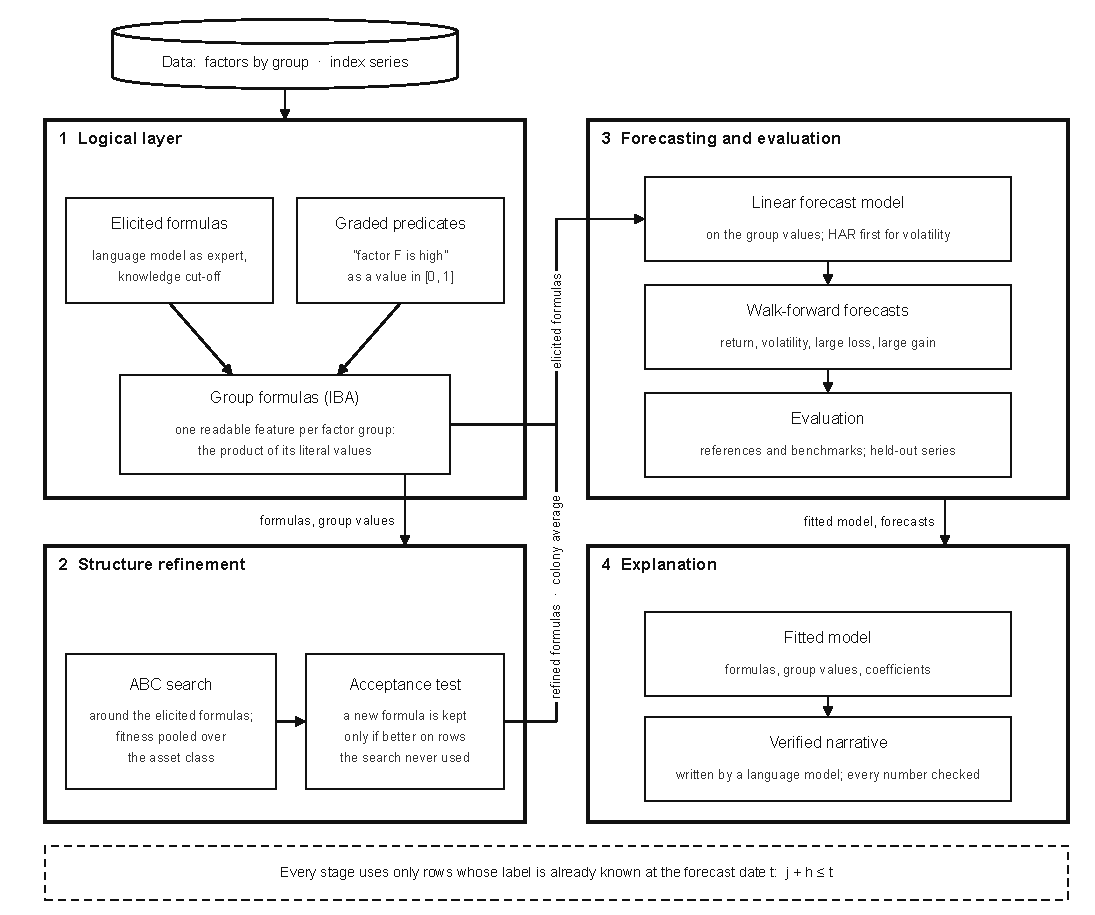
\includegraphics[width=\linewidth]{fig1_system_plain}
\caption{The IBA-based factor reduction framework.}\label{fig:1}
\end{figure}

\subsection{Predicates and Group Formulas}\label{sec:4.1}

Each factor enters as a trailing z-score: its current value against its own mean and standard deviation over the past 52 weeks (12 to 24 months for monthly data). The predicate ``factor F is high'' is this z-score scaled linearly to [0.01, 0.99] between its minimum and maximum in the training rows; its negation has the value 1 \ensuremath{-} x. Factors are arranged in eight economic groups (nine for monthly data; \ref{app:A}), and one further group holds the index's own recent behaviour. For each target, a group has one formula: a conjunction of at most two literals on different factors of the group, or none. Its value is the product of its literal values (Eq. 1). Table~\ref{tab:1} shows the formulas of one asset class. A formula names a state of its group; whether that state raises or lowers the target is left to the estimator. The logical layer therefore holds no fitted quantity, and a fitted sign that contradicts the reasoning behind a formula is visible.

{\small\setlength{\tabcolsep}{4pt}\renewcommand{\arraystretch}{1.2}
\begin{longtable}{@{}>{\raggedright\arraybackslash}p{0.372\linewidth}>{\raggedright\arraybackslash}p{0.597\linewidth}@{}}
\caption{Elicited formulas for broad US equity indices, target: volatility.}\label{tab:1}\\
\toprule
\textbf{Group} & \textbf{Formula} \\
\midrule
\endfirsthead
\toprule
\textbf{Group} & \textbf{Formula} \\
\midrule
\endhead
\bottomrule
\endlastfoot
Interest rates & 3-month T-bill rate change is NOT high \\
Credit & Baa credit spread change is high AND high-yield bond return is NOT high \\
Volatility & Equity VIX is high \\
Equity factors & Market excess return is NOT high \\
Styles & Short-term reversal is high \\
Currencies & USD/JPY return is NOT high \\
Commodities & Crude oil return is NOT high \\
Macro-financial conditions & Financial stress index is high \\
Own behaviour & Recent realised variance is high \\
\end{longtable}}


\subsection{Eliciting the Formulas}\label{sec:4.2}

The formulas are elicited from a large language model (Claude Opus 5.5, Anthropic) under a fixed protocol (\ref{app:B}). The model receives a manual that defines predicates, literals and formulas, the factors of each group and a description of the asset class, and returns for each target and group a formula with a short rationale. It is told that the date is 30 September 2017, one month before the first forecast of any series, and to use only what was known then. Each request is repeated five times, and the consensus formula keeps the literals given by more than half of the draws. A stated cut-off cannot be enforced, because the model was trained on later data. We limit and measure this risk in three ways: the formulas carry no direction and no parameter; two control sets are evaluated alongside, generic formulas shared by all asset classes and random formulas of the same shape; and a second procedure, which also shows the model training-sample correlations, could replace the first only by passing a pre-set test, which it did not.

\subsection{Forecast Model}\label{sec:4.3}

A ridge regression (return, volatility) or an L2-penalised logistic regression (tail events) maps the group values to the forecast. Volatility is fitted in two stages: a HAR regression on the index's own past variance, then the factor model on the HAR residual, so that the formulas are asked only for what HAR does not explain. We report two readings. The interpretable reading uses the consensus formulas. The accuracy reading averages the forecasts of the twenty formula sets of the final ABC colony. Gradient-boosted trees (LightGBM, XGBoost) are run on the same features as alternative estimators.

\subsection{Verified Explanations}\label{sec:4.4}

A language model writes a short explanation of a forecast, or of an asset class over the test period, from the exact numbers of the fitted model: the formulas with their rationales, each factor's degree of truth, each group's value, coefficient and contribution, and the measured track record. The text is accepted only if every number in it appears in that material; otherwise the request is repeated with the unmatched numbers named (\ref{app:F}).

\section{Experiments}\label{sec:5}

\subsection{Data}\label{sec:5.1}

The weekly series are 58 ETFs and indices with daily prices, June 2008 to September 2026, in eight asset classes: US equity (broad and sectors), developed and emerging markets, government and investment-grade bonds, high-yield and emerging-market debt, commodities and real estate. The monthly series are hedge-fund indices from 2005. The factors, four per group, come from FRED, the Kenneth French data library, the Fung--Hsieh trend-following factors and market data (\ref{app:A}).

The series were split once, before any model was run: 37 weekly series and 11 CISDM hedge-fund strategy indices for development, 21 weekly series for confirmation, at random within asset class. All choices of Sections~\ref{sec:3} and~\ref{sec:4} were made on the development series. The confirmation series were downloaded only after the method and the claims were fixed in writing, and the method was run on them once. For the hedge-fund indices we added, after the split, the 23 indices of a second provider (BarclayHedge) whose history covers the factor panel, and ran the frozen method on them once under claims of their own. Both confirmation sets cover the same years as the development data and are correlated with it: they test whether results depend on the series chosen, not whether they hold in a later period.

\subsection{Targets and References}\label{sec:5.2}

{\scriptsize\setlength{\tabcolsep}{4pt}\renewcommand{\arraystretch}{1.2}
\begin{longtable}{@{}>{\raggedright\arraybackslash}p{0.134\linewidth}>{\raggedright\arraybackslash}p{0.324\linewidth}>{\raggedright\arraybackslash}p{0.162\linewidth}>{\raggedright\arraybackslash}p{0.333\linewidth}@{}}
\caption{Targets and the references each forecast must outperform.}\label{tab:2}\\
\toprule
\textbf{Target} & \textbf{Definition (index, horizon h)} & \textbf{Primary loss} & \textbf{References} \\
\midrule
\endfirsthead
\toprule
\textbf{Target} & \textbf{Definition (index, horizon h)} & \textbf{Primary loss} & \textbf{References} \\
\midrule
\endhead
\bottomrule
\endlastfoot
Return & compounded return over the next h periods & squared error & \textbf{Historical mean:} the average h-period return of the index up to the forecast date. \textbf{Time-series momentum:} the index's return over the past year, scaled to h. \\
Volatility & log of realised variance (sum of squared daily log returns) over the next h weeks & squared error & \textbf{HAR:} regression of log variance on its values over the past 1, 4 and 13 weeks. \textbf{GARCH(1,1)} and \textbf{GJR-GARCH} on daily returns, aggregated to h weeks. \\
Large loss & return over h falls below the 10\,\% quantile of past returns & Brier score & \textbf{Base rate:} the event's frequency in the training data. \textbf{Volatility logit:} logistic regression on past realised variance. \textbf{GARCH probability:} probability of crossing the threshold under a normal distribution with GARCH variance. \\
Large gain & return over h rises above the 90\,\% quantile & Brier score & same three \\
\end{longtable}}


Horizons are 1, 4 and 13 weeks (4 and 13 for tail events), and 1, 3, 6 and 12 months for the hedge-fund indices (3 and 6 for tail events). Volatility is forecast for weekly series only.

\subsection{Protocol}\label{sec:5.3}

A data row holds the features at the end of period j and the label realised over j + 1, \ldots{}, j + h. At forecast date t, a row may enter any scaling, fit, tuning, threshold or selection only if j + h \ensuremath{\le} t. The test period is the last 416 weeks (96 months), in four blocks. At the start of a block, scalers, penalties and searched formulas are set on the rows admissible then, with five expanding validation folds separated from their training rows by the horizon; within a block the model is refitted every 4 weeks (every month). Every forecast is therefore made by a model that could have been built at its date (\ref{app:A}, Figure~\ref{fig:3}).

\subsection{Benchmarks, Tests and Claims}\label{sec:5.4}

The same factors are reduced by PCA and kernel PCA (six components each) and by an autoencoder with a six-unit bottleneck, and used without reduction (raw factors); a group-wise PCA and LASSO are reported in \ref{app:E}. Losses are the squared error for return and log variance and the Brier score for events. Series of one frequency share dates and shocks, so a comparison pools the series and resamples dates in blocks. We report the relative difference in loss with a 95\,\% bootstrap interval per task; ``significant'' means that the interval excludes zero.

Three claims were fixed before the weekly confirmation data were downloaded: a lower loss than HAR for volatility at 1 week and at 4 weeks (Holm-adjusted), and parity with group-wise PCA, the closest non-logical analogue of one formula per group. For the hedge-fund indices, where the development series had shown no advantage of any method, two claims of absence were fixed. \ref{app:C} lists all claims, their rules and their outcomes. The forecasts are also read in financial terms, declared in advance: value at risk from the variance forecast, and a timing rule that holds the index when the return forecast is not negative (\ref{app:E}).

\section{Results}\label{sec:6}

Entries are relative differences in the primary loss, pooled over series; negative favours the first-named method.

\subsection{Confirmation of the Claims}\label{sec:6.1}

All three claims for the weekly series are confirmed (Table~\ref{tab:3}), and so are the two for the hedge-fund indices: no factor method is significantly better than the reference in any of the eight tasks, and group-wise PCA is significantly better than the interpretable reading in one. The confirmation values are close to the development values; both sets cover the same period, so the same dates dominate both.

{\scriptsize\setlength{\tabcolsep}{4pt}\renewcommand{\arraystretch}{1.2}
\begin{longtable}{@{}>{\raggedright\arraybackslash}p{0.299\linewidth}>{\raggedright\arraybackslash}p{0.317\linewidth}>{\raggedright\arraybackslash}p{0.214\linewidth}>{\raggedright\arraybackslash}p{0.123\linewidth}@{}}
\caption{Claims for the weekly series, fixed before the confirmation data were downloaded.}\label{tab:3}\\
\toprule
\textbf{Claim} & \textbf{Confirmation (21 series)} & \textbf{Development (37 series)} & \textbf{Decision} \\
\midrule
\endfirsthead
\toprule
\textbf{Claim} & \textbf{Confirmation (21 series)} & \textbf{Development (37 series)} & \textbf{Decision} \\
\midrule
\endhead
\bottomrule
\endlastfoot
Volatility, 1 week: lower loss than HAR & \ensuremath{-}8.3\,\% (\ensuremath{-}12.7~to~\ensuremath{-}4.6), adjusted p < 0.001 & \ensuremath{-}7.2\,\% (\ensuremath{-}11.6~to~\ensuremath{-}3.8) & Confirmed \\
Volatility, 4 weeks: lower loss than HAR & \ensuremath{-}8.8\,\% (\ensuremath{-}17.6~to~\ensuremath{-}3.4), adjusted p = 0.024 & \ensuremath{-}7.8\,\% (\ensuremath{-}15.7~to~\ensuremath{-}2.7) & Confirmed \\
Parity with group PCA (upper bound below +3\,\% in at least 9 of 10 tasks; group PCA significantly better in none) & 10 of 10 tasks; largest upper bound +1.6\,\%; mean difference \ensuremath{-}0.7\,\% & 10 of 10; +1.4\,\%; \ensuremath{-}0.6\,\% & Confirmed \\
\end{longtable}}


\subsection{Accuracy by Target}\label{sec:6.2}

{\scriptsize\setlength{\tabcolsep}{4pt}\renewcommand{\arraystretch}{1.2}
\begin{longtable}{@{}>{\raggedright\arraybackslash}p{0.303\linewidth}>{\raggedright\arraybackslash}p{0.171\linewidth}>{\raggedright\arraybackslash}p{0.171\linewidth}>{\raggedleft\arraybackslash}p{0.150\linewidth}>{\raggedleft\arraybackslash}p{0.150\linewidth}@{}}
\caption{Loss relative to the reference (historical mean, HAR, base rate): 21 confirmation series, 37 development series in brackets.}\label{tab:4}\\
\toprule
\textbf{Method} & \textbf{Return} & \textbf{Volatility} & \textbf{Large loss} & \textbf{Large gain} \\
\midrule
\endfirsthead
\toprule
\textbf{Method} & \textbf{Return} & \textbf{Volatility} & \textbf{Large loss} & \textbf{Large gain} \\
\midrule
\endhead
\bottomrule
\endlastfoot
IBA, interpretable reading & +1.5\,\% (+1.0) & \textbf{\ensuremath{-}6.7\,\%} (\ensuremath{-}5.9) & +0.4\,\% (+0.8) & \ensuremath{-}1.5\,\% (\ensuremath{-}1.1) \\
IBA, accuracy reading & +1.2\,\% (+0.8) & \textbf{\ensuremath{-}6.8\,\%} (\ensuremath{-}6.0) & +0.2\,\% (+0.6) & \ensuremath{-}1.6\,\% (\ensuremath{-}1.2) \\
PCA & +1.1\,\% (+1.0) & \ensuremath{-}3.9\,\% (\ensuremath{-}3.5) & +0.6\,\% (+1.1) & \ensuremath{-}1.1\,\% (\ensuremath{-}0.5) \\
Raw factors & +3.6\,\% (+2.9) & \ensuremath{-}5.2\,\% (\ensuremath{-}4.7) & +1.1\,\% (+1.6) & +0.3\,\% (\ensuremath{-}0.1) \\
Kernel PCA & +0.7\,\% (+0.6) & \ensuremath{-}1.5\,\% (\ensuremath{-}1.3) & +0.7\,\% (+0.8) & 0.0\,\% (\ensuremath{-}0.2) \\
Autoencoder & +0.9\,\% (+0.9) & \ensuremath{-}3.3\,\% (\ensuremath{-}3.0) & +0.6\,\% (+0.9) & \ensuremath{-}1.1\,\% (\ensuremath{-}0.8) \\
Time-series momentum & +15.1\,\% (+12.1) & -- & -- & -- \\
GARCH(1,1) / GARCH probability & -- & +12.9\,\% (+10.7) & +3.2\,\% (+1.6) & \ensuremath{-}6.4\,\% (\ensuremath{-}4.6) \\
Volatility logit & -- & -- & +1.6\,\% (+1.7) & \ensuremath{-}5.8\,\% (\ensuremath{-}5.3) \\
\end{longtable}}


Every reduction of the factor panel improves on HAR for volatility, and the IBA readings improve most (Table~\ref{tab:4}). The interpretable reading is significantly better than PCA, kernel PCA and the autoencoder at all three horizons, by 2.9\,\%, 5.3\,\% and 3.5\,\% on average, and none of the three is significantly better than it in any return or tail task. Group-wise PCA is the closest competitor, about 1\,\% behind on volatility (\ref{app:E}). No method outperforms the historical mean on returns or the base rate on large losses. For large gains the IBA readings gain about 1.5\,\%, and the volatility-based references about 6\,\%: recent volatility says more about a large gain than the factor states do. Tree ensembles on the same features are worse than the linear model, by 3 to 7\,\% on IBA features.

On the hedge-fund indices of both providers no method has an advantage over the reference. On the 23 held-out indices the interpretable reading is 0.8\,\% behind the historical mean on returns and 2.6\,\% and 0.7\,\% behind the base rate for large losses and large gains.

The content of the formulas matters where there is signal. On volatility the elicited formulas are 2 to 5\,\% better than random formulas of the same shape at every horizon; on returns and large losses elicited, generic and random formulas cannot be told apart. Elicited and generic formulas perform alike although they share only a fifth of their literals: several sensible descriptions of a group's state work equally well (\ref{app:D}).

\subsection{Volatility and Extreme Events}\label{sec:6.3}

{\scriptsize\setlength{\tabcolsep}{4pt}\renewcommand{\arraystretch}{1.2}
\begin{longtable}{@{}>{\raggedright\arraybackslash}p{0.267\linewidth}>{\raggedright\arraybackslash}p{0.225\linewidth}>{\raggedright\arraybackslash}p{0.225\linewidth}>{\raggedright\arraybackslash}p{0.236\linewidth}@{}}
\caption{Volatility by horizon, confirmation series: squared error against HAR (95\,\% interval).}\label{tab:5}\\
\toprule
\textbf{Method} & \textbf{1 week} & \textbf{4 weeks} & \textbf{13 weeks} \\
\midrule
\endfirsthead
\toprule
\textbf{Method} & \textbf{1 week} & \textbf{4 weeks} & \textbf{13 weeks} \\
\midrule
\endhead
\bottomrule
\endlastfoot
IBA, interpretable reading & \ensuremath{-}8.3\,\% (\ensuremath{-}12.7~to~\ensuremath{-}4.6) & \ensuremath{-}8.8\,\% (\ensuremath{-}17.6~to~\ensuremath{-}3.4) & \ensuremath{-}3.1\,\% (\ensuremath{-}7.5~to~\ensuremath{-}0.2) \\
IBA, accuracy reading & \ensuremath{-}8.5\,\% (\ensuremath{-}12.8~to~\ensuremath{-}4.9) & \ensuremath{-}8.8\,\% (\ensuremath{-}17.0~to~\ensuremath{-}3.7) & \ensuremath{-}3.1\,\% (\ensuremath{-}7.0~to~\ensuremath{-}0.6) \\
Raw factors & \ensuremath{-}8.0\,\% (\ensuremath{-}13.2~to~\ensuremath{-}3.9) & \ensuremath{-}7.1\,\% (\ensuremath{-}16.8~to~\ensuremath{-}0.9) & \ensuremath{-}0.3\,\% (\ensuremath{-}5.1~to~+3.8) \\
PCA & \ensuremath{-}6.1\,\% (\ensuremath{-}10.2~to~\ensuremath{-}2.6) & \ensuremath{-}4.9\,\% (\ensuremath{-}10.9~to~\ensuremath{-}0.8) & \ensuremath{-}0.8\,\% (\ensuremath{-}3.3~to~+0.8) \\
Autoencoder & \ensuremath{-}5.4\,\% (\ensuremath{-}9.0~to~\ensuremath{-}2.4) & \ensuremath{-}4.0\,\% (\ensuremath{-}8.9~to~\ensuremath{-}0.6) & \ensuremath{-}0.6\,\% (\ensuremath{-}2.7~to~+0.9) \\
Kernel PCA & \ensuremath{-}3.3\,\% (\ensuremath{-}5.3~to~\ensuremath{-}1.4) & \ensuremath{-}1.3\,\% (\ensuremath{-}2.6~to~\ensuremath{-}0.1) & 0.0\,\% (\ensuremath{-}0.9~to~+0.9) \\
GARCH(1,1) & +15.2\,\% (+7.4~to~+21.9) & +10.9\,\% (\ensuremath{-}6.2~to~+23.3) & +12.5\,\% (\ensuremath{-}15.9~to~+33.4) \\
\end{longtable}}


At one week IBA and raw factors are equally good. The advantage of the formulas appears as the horizon grows: at 13 weeks they are the only reduction whose interval excludes zero, narrowly. The gain is largest for equity indices (about \ensuremath{-}10\,\%) and smallest for bonds (\ensuremath{-}1\,\%). Under QLIKE, which scores the level of the variance and not its logarithm, the result against HAR is the same, but GARCH is the stronger model at 4 and 13 weeks (\ref{app:E}); our claims are for the log variance, the loss fixed in advance.

The advantage is not uniform over time. On the confirmation series it is 18.8\,\% in the COVID-19 crash, 3.3\,\% in 2022 and 5.3\,\% outside the named periods, while in the sell-off of late 2018 the interpretable reading is 2.5\,\% worse than HAR. Figure~\ref{fig:2} follows one development series, the S\&P 500 fund SPY, through two of these episodes at the one-week horizon.

\begin{figure}[htbp]
\centering
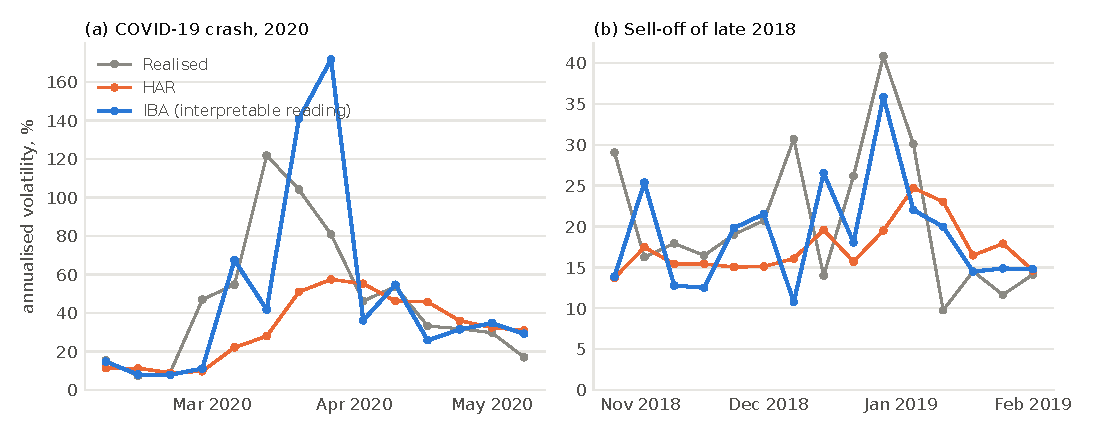
\includegraphics[width=\linewidth]{fig_crisis}
\caption{One-week volatility of SPY (a development series) in two stress episodes: realised value, HAR forecast and the interpretable reading. Every forecast is out of sample.}\label{fig:2}
\end{figure}

No model saw the first week of the crash: on 21 February 2020 HAR forecast an annualised volatility of 10\,\% and the interpretable reading 11\,\%, and 47\,\% was realised. One week later the statements had switched on. ``Market excess return is NOT high'' held to degree 0.99, ``VIX is high'' to 0.86 and ``credit spreads widen AND high-yield returns are NOT high'' to 0.90. They added 1.17, 1.03 and 0.57 to the forecast of log variance, the statement about the index's own variance took 0.65 back, and the forecast rose to 67\,\% against 22\,\% for HAR; 55\,\% was realised. The statements also switch off faster. After the rebound at the end of March the equity statement fell to 0.01 and the forecast to 36\,\%, below HAR's 55\,\%; 46\,\% was realised. In between the reading overshot: it forecast 141\,\% and 172\,\% for weeks that realised 104\,\% and 81\,\%. Over the ten weeks its squared error was 35\,\% below HAR's. The sign of the own-variance statement is negative in every forecast of the test period: its rationale expected persistence, but persistence is already in the HAR stage, and what the formula adds is mean reversion. Because each feature is a readable statement, such a disagreement between the expert's reasoning and the data is in plain sight.

The sell-off of late 2018 shows the cost of reacting fast. A one-week rally at the end of November switched the equity statement off (degree 0.12), the forecast fell to 11\,\%, and the following week realised 31\,\%. Over that quarter the reading was level with HAR for this series.

\subsection{Financial Reading}\label{sec:6.4}

A better variance forecast gives a better tail quantile at short horizons: at one week the 1\,\% value at risk from the interpretable reading has a 7.9\,\% lower quantile loss than HAR's (significant), and the 5\,\% value at risk a 3.6\,\% lower one (\ref{app:E}).

As secondary evidence, the timing rule on the one-week return forecasts has a Sharpe ratio of 0.68 against 0.56 for buy-and-hold on the confirmation series, higher in 16 of the 21, and a maximum drawdown of 25\,\% against 38\,\%; the development series show the same. We do not read this as a robust finding or as a trading rule. The rule changes position about twelve times a year, and at 10 basis points per switch the Sharpe ratio is 0.59 against 0.56. It works only at one week, it is out of the market a quarter of the time, which lowers drawdown by itself, and the test years include the sell-offs of 2020 and 2022, in which the series fall together. The return forecasts themselves are no more accurate than the historical mean, and on the held-out hedge-fund indices the same rule is ahead in only 12 of 23 series.

\subsection{Structure Search}\label{sec:6.5}

{\scriptsize\setlength{\tabcolsep}{4pt}\renewcommand{\arraystretch}{1.2}
\begin{longtable}{@{}>{\raggedright\arraybackslash}p{0.209\linewidth}>{\raggedright\arraybackslash}p{0.228\linewidth}>{\raggedright\arraybackslash}p{0.232\linewidth}>{\raggedright\arraybackslash}p{0.284\linewidth}@{}}
\caption{Structure search on the development series.}\label{tab:6}\\
\toprule
\textbf{Search} & \textbf{Gain on the selection folds} & \textbf{Gain on unused rows} & \textbf{Winners passing the acceptance test} \\
\midrule
\endfirsthead
\toprule
\textbf{Search} & \textbf{Gain on the selection folds} & \textbf{Gain on unused rows} & \textbf{Winners passing the acceptance test} \\
\midrule
\endhead
\bottomrule
\endlastfoot
ABC & +9.0\,\% & \ensuremath{-}1.4\,\% & 12\,\% \\
Genetic algorithm & +11.0\,\% & \ensuremath{-}2.0\,\% & 12\,\% \\
Particle swarm & +9.8\,\% & \ensuremath{-}2.0\,\% & 12\,\% \\
Simulated annealing & +9.7\,\% & \ensuremath{-}1.5\,\% & 12\,\% \\
Differential evolution & +10.5\,\% & \ensuremath{-}1.4\,\% & 13\,\% \\
\end{longtable}}

{\scriptsize\setlength{\tabcolsep}{4pt}\renewcommand{\arraystretch}{1.2}
\begin{longtable}{@{}>{\raggedright\arraybackslash}p{0.392\linewidth}>{\raggedleft\arraybackslash}p{0.090\linewidth}>{\raggedleft\arraybackslash}p{0.133\linewidth}>{\raggedleft\arraybackslash}p{0.133\linewidth}>{\raggedleft\arraybackslash}p{0.133\linewidth}@{}}
\toprule
\textbf{Forecasts against the fixed formula} & \textbf{Return} & \textbf{Volatility} & \textbf{Large loss} & \textbf{Large gain} \\
\midrule
\endfirsthead
\toprule
\textbf{Forecasts against the fixed formula} & \textbf{Return} & \textbf{Volatility} & \textbf{Large loss} & \textbf{Large gain} \\
\midrule
\endhead
\bottomrule
\endlastfoot
Exhaustive search over atoms & +8.3\,\% & +6.1\,\% & +12.7\,\% & +9.7\,\% \\
ABC winner, untested & +2.4\,\% & +1.5\,\% & +2.9\,\% & +2.7\,\% \\
ABC winner, after the acceptance test & +0.1\,\% & +0.3\,\% & +0.4\,\% & 0.0\,\% \\
ABC colony, averaged & \ensuremath{-}0.5\,\% & \ensuremath{-}0.2\,\% & \ensuremath{-}0.3\,\% & \ensuremath{-}0.1\,\% \\
\end{longtable}}
\addtocounter{table}{-1}


Search fits the selection data and does not transfer (Table~\ref{tab:6}). The five algorithms differ in how strongly they fit the selection folds and not in what remains on rows the search never saw; none is better than ABC, and a winner passes the acceptance test in about one search in eight. The more freely a search can choose, the worse its forecasts: exhaustive search over atoms is 6 to 13\,\% worse than the fixed formula. The acceptance test removes most of the damage and yields no gain. What survives is averaging: the colony ensemble is better than the fixed formula in 7 of 18 development tasks and worse in none, by a few tenths of a per cent, and better than the interpretable reading in 2 of 10 confirmation tasks. Wider search spaces, including graded formulas, fitted more and forecast worse (\ref{app:D}).

\section{Discussion and Conclusion}\label{sec:7}

Interpretability by construction cost nothing measurable. One short logical formula per factor group, elicited under a knowledge cut-off that precedes the test period, forecasts volatility better than PCA, kernel PCA and an autoencoder and is not worse than any of them on the other targets; against a group-wise PCA it is at parity, as claimed in advance. What it buys is a model whose every input is a sentence that the modeller, the risk manager and the supervisor can each check against the market, as the crisis weeks of Section~\ref{sec:6.3} show.

The method helps on risk, not on return. Volatility forecasts improve on HAR by 8 to 9\,\% at one and four weeks, most in equity markets, and at one week the improvement carries over to value at risk. Returns stay unpredictable and large losses stay at their base rate for every method, on ETFs and on the hedge-fund indices of two providers. Most of the gain over HAR comes from adding the factors at all; the logical form adds a little at longer horizons and makes the model legible. Content matters only where there is signal, and formulas with different wording but similar economic sense perform alike, so the method does not depend on the particular expert, human or machine, who writes them. Search over logical structures finds the noise of the validation data before it finds structure: for IBA models learned from data, fitness on the sample that guides the search is not evidence of forecasting value.

The limits are these. The confirmation series cover the same years as the development series and move with them, and the held-out hedge-fund indices average many of the same funds as the development ones; the runs show independence from the choice of series and provider, not stability over time. The language model was trained on data later than its stated cut-off, and the formulas were elicited after the test period had ended; that elicited formulas do not outperform random ones on returns argues against a large hindsight effect but cannot exclude one. The volatility claims are for the logarithm of realised variance, and value at risk uses a normal distribution. Future work is a test on later data, formulas with disjunctions, and explanations evaluated by the people who would use them.

Factor reduction for financial forecasting does not have to be opaque. A handful of logical statements about named groups of factors, elicited from a language model and combined by Interpolative Boolean Algebra, matches the accuracy of standard reductions, improves volatility and value-at-risk forecasts over HAR on held-out indices, and lets every forecast be traced to the state of the market that produced it.

\appendix
\renewcommand{\baselinestretch}{1.0}\small

\section{Data and protocol}\label{app:A}

\setcounter{table}{0}

{\scriptsize\setlength{\tabcolsep}{4pt}\renewcommand{\arraystretch}{1.2}
\begin{longtable}{@{}>{\raggedright\arraybackslash}p{0.305\linewidth}>{\raggedright\arraybackslash}p{0.321\linewidth}>{\raggedright\arraybackslash}p{0.335\linewidth}@{}}
\caption{Index series by asset class and role.}\label{tab:A1}\\
\toprule
\textbf{Asset class} & \textbf{Development series} & \textbf{Confirmation series} \\
\midrule
\endfirsthead
\toprule
\textbf{Asset class} & \textbf{Development series} & \textbf{Confirmation series} \\
\midrule
\endhead
\bottomrule
\endlastfoot
US equity, broad & DIA, IWM, SPY & MDY, QQQ \\
US equity, sectors & XLE, XLI, XLP, XLV, XLY & XLB, XLF, XLK, XLU \\
Developed markets ex-US & EFA, EWG, EWH, EWI, EWL, EWN, EWP, EWQ & EWA, EWC, EWD, EWJ, EWS, EWU \\
Emerging markets & EEM, EWT, EWY, EZA, FXI & EWW, EWZ \\
Government and investment-grade bonds & AGG, BND, IEF, TIP, TLT & LQD, MUB, SHY \\
High-yield and emerging-market debt & EMB, HYG & -- \\
Commodities & DBA, DBB, DBC, DBE, GLD, GSG, SLV, UNG & DBP, USO, \textasciicircum{}SPGSCI \\
Real estate & VNQ & IYR \\
Hedge-fund strategy indices (monthly) & CA, CTA, DS, EDMS, ELS, EMN, EWHF, FIA, FOF, GM, MA & BarclayHedge indices: Convertible Arbitrage, Distressed Securities, Emerging Markets, Emerging Markets Asia, Emerging Markets Asian Equities, Emerging Markets Eastern Europe, Emerging Markets Global Equities, Emerging Markets Latin America, Equity Long Bias, Equity Long/Short, Equity Market Neutral, European Equities, Event Driven, Fixed Income Arbitrage, Fund of Funds, Global Macro, Healthcare \& Biotechnology, Hedge Fund, Merger Arbitrage, Multi Strategy, Option Strategies, Pacific Rim Equities, Technology \\
\end{longtable}}


{\scriptsize\setlength{\tabcolsep}{4pt}\renewcommand{\arraystretch}{1.2}
\begin{longtable}{@{}>{\raggedright\arraybackslash}p{0.247\linewidth}>{\raggedright\arraybackslash}p{0.355\linewidth}>{\raggedright\arraybackslash}p{0.359\linewidth}@{}}
\caption{Factor groups (four factors each).}\label{tab:A2}\\
\toprule
\textbf{Group} & \textbf{Weekly factors} & \textbf{Monthly factors} \\
\midrule
\endfirsthead
\toprule
\textbf{Group} & \textbf{Weekly factors} & \textbf{Monthly factors} \\
\midrule
\endhead
\bottomrule
\endlastfoot
Interest rates & changes in the 3-month bill rate, the 10y--2y spread, the 1y and 5y spreads to Fed Funds & same \\
Credit & Baa and Aaa spread changes; high-yield and EM sovereign bond returns & yield changes: US AAA, US single-B, euro high-yield, EM corporate \\
Volatility & VIX, oil and gold implied volatility, policy uncertainty & VIX; commodity, financial-crisis and macro volatility trackers \\
Equity factors & market, size, value, emerging-market equity & same \\
Styles & momentum, profitability, investment, short-term reversal & same \\
Currencies & EUR/USD, USD/JPY, AUD/USD, broad dollar & EUR/USD, USD/JPY, AUD/USD, currency trend factor \\
Commodities & oil, natural gas, broad commodities, silver & oil, natural gas, copper, all-commodity index \\
Macro-financial conditions & financial conditions, financial stress, jobless claims, inflation expectations & financial conditions, financial stress, economic activity, inflation expectations \\
Trend-following & --- & bond, commodity, short-rate and stock trend factors \\
\end{longtable}}


Weekly series: adjusted daily closes; realised variance is the sum of squared daily log returns within the week. The BarclayHedge indices are every index of that provider with a monthly history over the whole factor panel, 23 of the 26 that could be obtained; their September 2026 value is the provider's estimate. Two daily trend-following indices assigned to confirmation at the split could not be obtained and were not run. Protocol settings (weekly; monthly): test period 416 weeks; 96 months. Re-selection every 104; 24. Refit every 4; 1. Validation folds 5 \ensuremath{\times} 78; 5 \ensuremath{\times} 18. Minimum training sample 300; 110.

\begin{figure}[htbp]
\centering
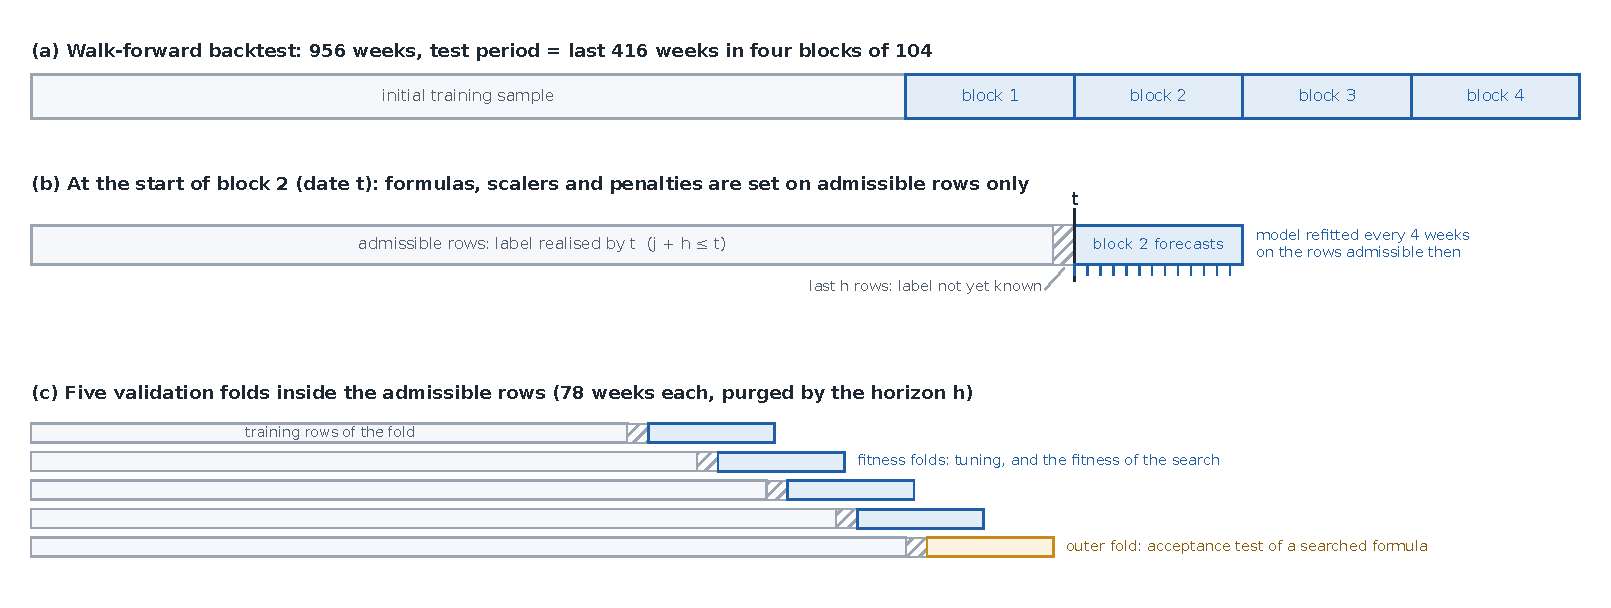
\includegraphics[width=\linewidth]{fig2_backtest}
\caption{Walk-forward backtest (a), the information available at a block start (b), and the validation folds (c). Weekly protocol shown.}\label{fig:3}
\end{figure}

\section{Elicitation of the formulas}\label{app:B}

\setcounter{table}{0}

The model (requests of 14 November 2026) receives the role of a senior researcher in macro-finance; the instruction that the date is 30 September 2017 and that nothing later may be used; a manual of about 600 words that defines predicate, literal and formula and states that a formula describes a state of its group and not its effect on the target; the factors of each group; and a description of the asset class. The second procedure adds rank correlations between each factor and each target, computed on rows before the first forecast date. An answer is rejected and requested again if a factor is not in its group, a group has more than two literals, or the text mentions a year after 2017. All 95 requests were valid at the first attempt. The five draws of a procedure share 0.69 of their literals on average (Jaccard index); the consensus keeps 20\,\% of the literals of the generic formula set. Every request, answer and rationale, and the formulas of every asset class and target, are in the repository.

\section{Claims and decision rules}\label{app:C}

\setcounter{table}{0}

The claims, their rules and the tests were fixed in specifications that were frozen before the confirmation series were used. A primary claim is confirmed or not by its rule; a secondary claim holds or does not hold and cannot rescue a primary one. Each run was made once, and no deviation was recorded. For the hedge-fund indices the 3\,\% parity margin of the weekly claims was not claimed, because the development intervals were too wide to support it.

{\scriptsize\setlength{\tabcolsep}{4pt}\renewcommand{\arraystretch}{1.2}
\begin{longtable}{@{}>{\raggedright\arraybackslash}p{0.069\linewidth}>{\raggedright\arraybackslash}p{0.226\linewidth}>{\raggedright\arraybackslash}p{0.254\linewidth}>{\raggedright\arraybackslash}p{0.141\linewidth}>{\raggedright\arraybackslash}p{0.254\linewidth}@{}}
\caption{Claims for the weekly series, with the same quantity on the development series.}\label{tab:C1}\\
\toprule
\textbf{Claim} & \textbf{Statement} & \textbf{Result} & \textbf{Decision} & \textbf{Development (weekly series; decisions were not made there)} \\
\midrule
\endfirsthead
\toprule
\textbf{Claim} & \textbf{Statement} & \textbf{Result} & \textbf{Decision} & \textbf{Development (weekly series; decisions were not made there)} \\
\midrule
\endhead
\bottomrule
\endlastfoot
P1 & Volatility at 1 week: interpretable reading better than HAR & \ensuremath{-}8.3\,\% (\ensuremath{-}12.7~to~\ensuremath{-}4.6), p < 0.001; Holm-adjusted p < 0.001 & CONFIRMED & \ensuremath{-}7.2\,\% (\ensuremath{-}11.6~to~\ensuremath{-}3.8), p < 0.001; Holm-adjusted p < 0.001 \\
P2 & Volatility at 4 weeks: interpretable reading better than HAR & \ensuremath{-}8.8\,\% (\ensuremath{-}17.6~to~\ensuremath{-}3.4), p = 0.024; Holm-adjusted p = 0.024 & CONFIRMED & \ensuremath{-}7.8\,\% (\ensuremath{-}15.7~to~\ensuremath{-}2.7), p = 0.028; Holm-adjusted p = 0.028 \\
P3 & Parity with group PCA: upper end of the interval below +3\,\% in at least 9 of 10 tasks, group PCA significantly better in none & below the margin in 10 of 10; group PCA significantly better in 0; mean difference \ensuremath{-}0.73\,\%; largest upper end +1.62\,\% & CONFIRMED & below the margin in 10 of 10; group PCA significantly better in 0; mean difference \ensuremath{-}0.64\,\%; largest upper end +1.44\,\% \\
S1 & Volatility at 13 weeks against HAR (no~direction~claimed) & \ensuremath{-}3.1\,\% (\ensuremath{-}7.5~to~\ensuremath{-}0.2), p = 0.080 & reported & \ensuremath{-}2.5\,\% (\ensuremath{-}6.0~to~\ensuremath{-}0.2), p = 0.074 \\
S2 & Accuracy reading better than the interpretable one in more tasks than worse & \ensuremath{-}0.17\,\% (2~better,~0~worse~of~10) & holds & \ensuremath{-}0.18\,\% (5~better,~0~worse~of~10) \\
S3 & On volatility the interpretable reading is better than PCA, kernel PCA and the autoencoder in at least 2 of 3 horizons each & PCA: \ensuremath{-}2.95\,\% (3~better,~0~worse~of~3); kernel PCA: \ensuremath{-}5.31\,\% (3~better,~0~worse~of~3); autoencoder: \ensuremath{-}3.53\,\% (3~better,~0~worse~of~3) & holds & PCA: not available; kernel PCA: \ensuremath{-}4.66\,\% (3~better,~0~worse~of~3); autoencoder: \ensuremath{-}3.00\,\% (3~better,~0~worse~of~3) \\
S4 & Against random formulas: better on volatility in at least 2 of 3 horizons; at most 1 significant difference in the return and tail tasks & volatility: \ensuremath{-}3.77\,\% (3~better,~0~worse~of~3); returns and tails: +0.07\,\% (0~better,~0~worse~of~7) & holds & volatility: \ensuremath{-}3.36\,\% (3~better,~0~worse~of~3); returns and tails: +0.01\,\% (1~better,~0~worse~of~7) \\
S5 & No factor method is significantly better than the reference in any return or large-loss task & none & holds & none \\
S6 & Elicited and generic formulas at parity: at most 1 task with a significant difference & \ensuremath{-}0.62\,\% (1~better,~0~worse~of~10) & holds & \ensuremath{-}0.31\,\% (0~better,~0~worse~of~10) \\
S7 & Trees do not help: XGBoost and LightGBM significantly worse than the linear model in more tasks than better (IBA, raw factors, group PCA) & IBA + XGBoost: 0 better, 9 worse of 10; IBA + LightGBM: 0 better, 8 worse of 10; raw factors + XGBoost: 0 better, 7 worse of 10; raw factors + LightGBM: 0 better, 7 worse of 10; group PCA + XGBoost: 0 better, 10 worse of 10; group PCA + LightGBM: 0 better, 10 worse of 10 & holds & IBA + XGBoost: 0 better, 10 worse of 10; IBA + LightGBM: 0 better, 9 worse of 10; raw factors + XGBoost: 0 better, 8 worse of 10; raw factors + LightGBM: 0 better, 7 worse of 10; group PCA + XGBoost: 0 better, 10 worse of 10; group PCA + LightGBM: 0 better, 10 worse of 10 \\
S8 & Large gains: the volatility-based logit has the lower loss than the interpretable reading in every large-gain task & large gain, 13 weeks: \ensuremath{-}5.1\,\%; large gain, 4 weeks: \ensuremath{-}3.5\,\% & holds & not available \\
S9 & One-week 1\,\% value at risk: lower quantile loss than HAR & \ensuremath{-}7.9\,\% (better) & holds &  \\
S10 & Long/flat rule at one week: higher Sharpe ratio than buy-and-hold in at least 15 of 21 series, and a smaller maximum drawdown in at least 15 & Sharpe 0.68 against 0.56, higher in 16; drawdown 24.6\,\% against 37.7\,\%, smaller in 17; after 10 bp per switch Sharpe 0.59 against 0.56, higher in 11 & holds &  \\
S11 & Large gains as a classifier: Matthews correlation below that of the volatility-based logit & 0.106 against 0.183 & holds &  \\
\end{longtable}}


{\scriptsize\setlength{\tabcolsep}{4pt}\renewcommand{\arraystretch}{1.2}
\begin{longtable}{@{}>{\raggedright\arraybackslash}p{0.069\linewidth}>{\raggedright\arraybackslash}p{0.226\linewidth}>{\raggedright\arraybackslash}p{0.254\linewidth}>{\raggedright\arraybackslash}p{0.141\linewidth}>{\raggedright\arraybackslash}p{0.254\linewidth}@{}}
\caption{Claims for the hedge-fund indices of the second provider, with the same quantity on the 11 development indices.}\label{tab:C2}\\
\toprule
\textbf{Claim} & \textbf{Statement} & \textbf{Result} & \textbf{Decision} & \textbf{Development (11 CISDM indices; decisions were not made there)} \\
\midrule
\endfirsthead
\toprule
\textbf{Claim} & \textbf{Statement} & \textbf{Result} & \textbf{Decision} & \textbf{Development (11 CISDM indices; decisions were not made there)} \\
\midrule
\endhead
\bottomrule
\endlastfoot
H1 & No factor method (the two IBA readings and the six reductions, linear model) is significantly better than the reference in any task & none & CONFIRMED & none \\
H2 & Group PCA is significantly better than the interpretable reading in at most 1 task & group PCA significantly better in 1 of 8; interpretable reading significantly better in 0; mean difference +0.68\,\%; upper end of the interval below +3\,\% in 4 of 8 (reported,~no~rule) & CONFIRMED & group PCA significantly better in 1 of 8; interpretable reading significantly better in 0; mean difference +1.10\,\%; upper end of the interval below +3\,\% in 4 of 8 (reported,~no~rule) \\
H3 & Accuracy reading better than the interpretable one in more tasks than worse & \ensuremath{-}0.52\,\% (1~better,~0~worse~of~8) & holds & \ensuremath{-}0.47\,\% (2~better,~0~worse~of~8) \\
H4 & Elicited formulas at parity with generic and with random formulas: at most 1 task with a significant difference against each & against generic: +0.07\,\% (0~better,~0~worse~of~8); against random: +0.06\,\% (0~better,~0~worse~of~8) & holds & against generic: +1.04\,\% (0~better,~0~worse~of~8); against random: +0.29\,\% (0~better,~0~worse~of~8) \\
H5 & Trees do not help: XGBoost and LightGBM significantly worse than the linear model in more tasks than better (IBA, raw factors, group PCA) & IBA + XGBoost: 0 better, 6 worse of 8; IBA + LightGBM: 0 better, 3 worse of 8; raw factors + XGBoost: 0 better, 4 worse of 8; raw factors + LightGBM: 0 better, 4 worse of 8; group PCA + XGBoost: 0 better, 4 worse of 8; group PCA + LightGBM: 0 better, 6 worse of 8 & holds & IBA + XGBoost: 0 better, 4 worse of 8; IBA + LightGBM: 0 better, 3 worse of 8; raw factors + XGBoost: 0 better, 4 worse of 8; raw factors + LightGBM: 0 better, 4 worse of 8; group PCA + XGBoost: 0 better, 4 worse of 8; group PCA + LightGBM: 0 better, 5 worse of 8 \\
H6 & The interpretable reading against the reference, by target (no~direction~claimed) & returns: +0.85\,\% (0~better,~0~worse~of~4); large losses: +2.58\,\% (0~better,~1~worse~of~2); large gains: +0.73\,\% (0~better,~0~worse~of~2) & reported & returns: +2.95\,\% (0~better,~1~worse~of~4); large losses: +0.08\,\% (0~better,~0~worse~of~2); large gains: +0.87\,\% (0~better,~1~worse~of~2) \\
\end{longtable}}


\section{Components, formula content and search}\label{app:D}

\setcounter{table}{0}

{\scriptsize\setlength{\tabcolsep}{4pt}\renewcommand{\arraystretch}{1.2}
\begin{longtable}{@{}>{\raggedright\arraybackslash}p{0.448\linewidth}>{\raggedleft\arraybackslash}p{0.090\linewidth}>{\raggedleft\arraybackslash}p{0.133\linewidth}>{\raggedleft\arraybackslash}p{0.133\linewidth}>{\raggedleft\arraybackslash}p{0.133\linewidth}@{}}
\caption{Loss relative to the reference as components are added (weekly development series).}\label{tab:D1}\\
\toprule
\textbf{Configuration} & \textbf{Return} & \textbf{Volatility} & \textbf{Large loss} & \textbf{Large gain} \\
\midrule
\endfirsthead
\toprule
\textbf{Configuration} & \textbf{Return} & \textbf{Volatility} & \textbf{Large loss} & \textbf{Large gain} \\
\midrule
\endhead
\bottomrule
\endlastfoot
Raw factors, no reduction & +2.9\,\% & \ensuremath{-}4.7\,\% & +1.6\,\% & \ensuremath{-}0.1\,\% \\
One feature per group: group PCA & +1.5\,\% & \ensuremath{-}4.9\,\% & +1.4\,\% & \ensuremath{-}0.6\,\% \\
Logical form, random content & +0.7\,\% & \ensuremath{-}2.6\,\% & +0.6\,\% & \ensuremath{-}0.5\,\% \\
Logical form, generic content & +1.0\,\% & \ensuremath{-}5.3\,\% & +0.8\,\% & \ensuremath{-}0.4\,\% \\
Logical form, elicited content (interpretable~reading) & +1.0\,\% & \ensuremath{-}5.9\,\% & +0.8\,\% & \ensuremath{-}1.1\,\% \\
+ averaging with random neighbours & +0.9\,\% & \ensuremath{-}6.0\,\% & +0.7\,\% & \ensuremath{-}1.1\,\% \\
+ averaging over the ABC colony (accuracy~reading) & +0.8\,\% & \ensuremath{-}6.0\,\% & +0.6\,\% & \ensuremath{-}1.2\,\% \\
\end{longtable}}


{\scriptsize\setlength{\tabcolsep}{4pt}\renewcommand{\arraystretch}{1.2}
\begin{longtable}{@{}>{\raggedright\arraybackslash}p{0.290\linewidth}>{\raggedright\arraybackslash}p{0.162\linewidth}>{\raggedright\arraybackslash}p{0.170\linewidth}>{\raggedright\arraybackslash}p{0.162\linewidth}>{\raggedright\arraybackslash}p{0.162\linewidth}@{}}
\caption{One component of the interpretable reading changed (weekly development series); positive = the component contributes.}\label{tab:D2}\\
\toprule
\textbf{Change} & \textbf{Return} & \textbf{Volatility} & \textbf{Large loss} & \textbf{Large gain} \\
\midrule
\endfirsthead
\toprule
\textbf{Change} & \textbf{Return} & \textbf{Volatility} & \textbf{Large loss} & \textbf{Large gain} \\
\midrule
\endhead
\bottomrule
\endlastfoot
Without interest rates & \ensuremath{-}0.0\,\% (0/0~of~3) & \ensuremath{-}0.1\,\% (0/0~of~3) & \ensuremath{-}0.1\,\% (0/0~of~2) & \ensuremath{-}0.1\,\% (0/0~of~2) \\
Without credit & +0.0\,\% (0/0~of~3) & +1.0\,\% (0/2~of~3) & \ensuremath{-}0.0\,\% (0/0~of~2) & \ensuremath{-}0.1\,\% (0/0~of~2) \\
Without volatility & \ensuremath{-}0.1\,\% (0/0~of~3) & +0.9\,\% (0/0~of~3) & \ensuremath{-}0.1\,\% (0/0~of~2) & +0.8\,\% (0/1~of~2) \\
Without equity factors & +0.1\,\% (0/1~of~3) & +0.4\,\% (0/0~of~3) & +0.0\,\% (0/0~of~2) & \ensuremath{-}0.1\,\% (0/0~of~2) \\
Without styles & \ensuremath{-}0.1\,\% (0/0~of~3) & +0.1\,\% (0/0~of~3) & +0.0\,\% (0/0~of~2) & \ensuremath{-}0.1\,\% (0/0~of~2) \\
Without currencies & +0.0\,\% (0/0~of~3) & \ensuremath{-}0.2\,\% (0/0~of~3) & \ensuremath{-}0.1\,\% (0/0~of~2) & \ensuremath{-}0.0\,\% (0/0~of~2) \\
Without commodities & +0.0\,\% (0/0~of~3) & \ensuremath{-}0.1\,\% (0/0~of~3) & +0.0\,\% (0/0~of~2) & \ensuremath{-}0.1\,\% (0/0~of~2) \\
Without macro-financial conditions & \ensuremath{-}0.5\,\% (0/0~of~3) & \ensuremath{-}0.4\,\% (2/0~of~3) & \ensuremath{-}0.2\,\% (0/0~of~2) & \ensuremath{-}0.0\,\% (1/0~of~2) \\
Without own behaviour & +0.0\,\% (0/1~of~3) & +1.9\,\% (0/3~of~3) & +0.0\,\% (0/0~of~2) & \ensuremath{-}0.0\,\% (0/0~of~2) \\
One literal per group & +0.0\,\% (0/0~of~3) & +0.4\,\% (0/0~of~3) & +0.1\,\% (0/0~of~2) & +0.2\,\% (0/0~of~2) \\
Distribution-based scaling & \ensuremath{-}0.3\,\% (0/0~of~3) & +1.3\,\% (0/0~of~3) & +0.1\,\% (0/0~of~2) & +0.0\,\% (0/0~of~2) \\
No HAR stage & -- & +27.5\,\% (0/2~of~3) & -- & -- \\
\end{longtable}}


For volatility, the group of the index's own behaviour and the credit group contribute significantly, and the HAR first stage is essential: without it the loss is 27.5\,\% higher. One literal per group against two, and the scaling of predicates, make no significant difference.

{\scriptsize\setlength{\tabcolsep}{4pt}\renewcommand{\arraystretch}{1.2}
\begin{longtable}{@{}>{\raggedright\arraybackslash}p{0.325\linewidth}>{\raggedleft\arraybackslash}p{0.089\linewidth}>{\raggedleft\arraybackslash}p{0.132\linewidth}>{\raggedleft\arraybackslash}p{0.102\linewidth}>{\raggedleft\arraybackslash}p{0.102\linewidth}>{\raggedright\arraybackslash}p{0.187\linewidth}@{}}
\caption{Elicited formulas against the two controls (interpretable reading).}\label{tab:D3}\\
\toprule
\textbf{Comparison} & \textbf{Return} & \textbf{Volatility} & \textbf{Large loss} & \textbf{Large gain} & \textbf{Significant tasks} \\
\midrule
\endfirsthead
\toprule
\textbf{Comparison} & \textbf{Return} & \textbf{Volatility} & \textbf{Large loss} & \textbf{Large gain} & \textbf{Significant tasks} \\
\midrule
\endhead
\bottomrule
\endlastfoot
Elicited vs generic, confirmation & 0.0\,\% & \ensuremath{-}1.2\,\% & +0.1\,\% & \ensuremath{-}1.4\,\% & 1 of 10 \\
Elicited vs random, confirmation & +0.6\,\% & \ensuremath{-}3.8\,\% & +0.2\,\% & \ensuremath{-}0.9\,\% & 3 of 10 (volatility) \\
Elicited vs generic, development & +0.7\,\% & \ensuremath{-}0.6\,\% & +0.7\,\% & \ensuremath{-}0.3\,\% & 0 of 18 \\
Elicited vs random, development & +0.9\,\% & \ensuremath{-}3.4\,\% & \ensuremath{-}0.4\,\% & \ensuremath{-}0.5\,\% & 4 of 18 \\
Statistics-informed (S) vs knowledge-only (K), development & \ensuremath{-}1.2\,\% & +0.1\,\% & \ensuremath{-}0.9\,\% & +0.5\,\% & 0 of 18 \\
\end{longtable}}


\textbf{Search.} All algorithms share the search space (at most three literals per group, at most four changes from the prior), the start, the pooled fitness, a budget of 2,000 distinct formula sets and three seeds. The acceptance test uses the rows of the fifth validation fold that no fitness fold used: the candidate is accepted if its mean gain over the prior on those dates exceeds the standard error of that gain, computed from non-overlapping blocks. Three wider variants of ABC were run on the development series: a colony started at random formula sets, moves that change the whole structure vector, and graded formulas in which each literal has a degree of inclusion. The gain on the selection folds rose from 14\,\% to 20\,\%, 25\,\% and 35\,\%; the winner's gain on unused rows fell from \ensuremath{-}6.7\,\% to \ensuremath{-}8.2\,\%, \ensuremath{-}11.3\,\% and \ensuremath{-}15.7\,\%.

\section{Additional results}\label{app:E}

\setcounter{table}{0}

Benchmark settings: PCA and kernel PCA (RBF kernel) with six components; group-wise PCA with the first component of each group; LASSO with a cross-validated penalty; an autoencoder with layers p--16--6--16--p, tanh activations, one seed. LightGBM and XGBoost: depth 2 or 4, 100 or 300 trees, no sampling. Value at risk: the quantile of a zero-mean normal return with the forecast variance. Timing rule: long the index for the next h periods when the forecast return is not negative, otherwise flat; cost variant with 10 basis points per change of position. Crisis periods, by forecast date: the fourth quarter of 2018; 17 February to 30 April 2020; 21 February to 31 October 2022.

\medskip\noindent \textbf{Confirmation, weekly}

{\scriptsize\setlength{\tabcolsep}{4pt}\renewcommand{\arraystretch}{1.2}
\begin{longtable}{@{}>{\raggedright\arraybackslash}p{0.243\linewidth}>{\raggedright\arraybackslash}p{0.179\linewidth}>{\raggedright\arraybackslash}p{0.180\linewidth}>{\raggedright\arraybackslash}p{0.171\linewidth}>{\raggedright\arraybackslash}p{0.171\linewidth}@{}}
\caption{Loss relative to the reference, every method, on the two confirmation sets. Entry: mean over tasks (tasks significantly better / worse).}\label{tab:E1}\\
\toprule
\textbf{Method} & \textbf{Return} & \textbf{Volatility} & \textbf{Large loss} & \textbf{Large gain} \\
\midrule
\endfirsthead
\toprule
\textbf{Method} & \textbf{Return} & \textbf{Volatility} & \textbf{Large loss} & \textbf{Large gain} \\
\midrule
\endhead
\bottomrule
\endlastfoot
IBA, interpretable reading & +1.5\,\% (0/0~of~3) & \ensuremath{-}6.7\,\% (3/0~of~3) & +0.4\,\% (0/1~of~2) & \ensuremath{-}1.5\,\% (1/0~of~2) \\
IBA, accuracy reading & +1.2\,\% (0/0~of~3) & \ensuremath{-}6.8\,\% (3/0~of~3) & +0.2\,\% (0/1~of~2) & \ensuremath{-}1.6\,\% (1/0~of~2) \\
IBA, generic formulas & +1.6\,\% (0/1~of~3) & \ensuremath{-}5.6\,\% (2/0~of~3) & +0.3\,\% (0/1~of~2) & \ensuremath{-}0.1\,\% (0/0~of~2) \\
IBA, random formulas & +0.9\,\% (0/1~of~3) & \ensuremath{-}3.1\,\% (2/0~of~3) & +0.3\,\% (0/0~of~2) & \ensuremath{-}0.6\,\% (0/0~of~2) \\
Group PCA & +2.1\,\% (0/2~of~3) & \ensuremath{-}5.5\,\% (2/0~of~3) & +0.8\,\% (0/1~of~2) & \ensuremath{-}1.0\,\% (1/0~of~2) \\
PCA & +1.1\,\% (0/2~of~3) & \ensuremath{-}3.9\,\% (2/0~of~3) & +0.6\,\% (0/1~of~2) & \ensuremath{-}1.1\,\% (1/0~of~2) \\
LASSO & +2.6\,\% (0/1~of~3) & \ensuremath{-}4.3\,\% (2/0~of~3) & +0.4\,\% (0/0~of~2) & \ensuremath{-}0.8\,\% (1/0~of~2) \\
Raw factors & +3.6\,\% (0/2~of~3) & \ensuremath{-}5.2\,\% (2/0~of~3) & +1.1\,\% (0/1~of~2) & +0.3\,\% (0/0~of~2) \\
Kernel PCA & +0.7\,\% (0/2~of~3) & \ensuremath{-}1.5\,\% (2/0~of~3) & +0.7\,\% (0/1~of~2) & \ensuremath{-}0.0\,\% (0/1~of~2) \\
Autoencoder & +0.9\,\% (0/2~of~3) & \ensuremath{-}3.3\,\% (2/0~of~3) & +0.6\,\% (0/1~of~2) & \ensuremath{-}1.1\,\% (1/0~of~2) \\
Time-series momentum & +15.1\,\% (0/3~of~3) & -- & -- & -- \\
GARCH(1,1) & -- & +12.9\,\% (0/1~of~3) & -- & -- \\
GJR-GARCH & -- & +7.7\,\% (0/1~of~3) & -- & -- \\
Volatility logit & -- & -- & +1.6\,\% (0/1~of~2) & \ensuremath{-}5.8\,\% (1/0~of~2) \\
GARCH probability & -- & -- & +3.2\,\% (0/0~of~2) & \ensuremath{-}6.4\,\% (1/0~of~2) \\
\end{longtable}}

{\scriptsize\setlength{\tabcolsep}{4pt}\renewcommand{\arraystretch}{1.2}
\begin{longtable}{@{}>{\raggedright\arraybackslash}p{0.223\linewidth}>{\raggedright\arraybackslash}p{0.204\linewidth}>{\raggedright\arraybackslash}p{0.133\linewidth}>{\raggedright\arraybackslash}p{0.193\linewidth}>{\raggedright\arraybackslash}p{0.193\linewidth}@{}}
\toprule
\textbf{Method} & \textbf{Return} & \textbf{Volatility} & \textbf{Large loss} & \textbf{Large gain} \\
\midrule
\endfirsthead
\toprule
\textbf{Method} & \textbf{Return} & \textbf{Volatility} & \textbf{Large loss} & \textbf{Large gain} \\
\midrule
\endhead
\bottomrule
\endlastfoot
IBA, interpretable reading & +0.8\,\% (0/0~of~4) & -- & +2.6\,\% (0/1~of~2) & +0.7\,\% (0/0~of~2) \\
IBA, accuracy reading & +0.6\,\% (0/0~of~4) & -- & +1.5\,\% (0/0~of~2) & +0.3\,\% (0/0~of~2) \\
IBA, generic formulas & +1.0\,\% (0/0~of~4) & -- & +1.2\,\% (0/0~of~2) & +1.6\,\% (0/2~of~2) \\
IBA, random formulas & +1.2\,\% (0/0~of~4) & -- & +1.1\,\% (0/1~of~2) & +1.3\,\% (0/2~of~2) \\
Group PCA & +0.7\,\% (0/0~of~4) & -- & +0.2\,\% (0/0~of~2) & +0.6\,\% (0/1~of~2) \\
PCA & +1.6\,\% (0/0~of~4) & -- & +0.8\,\% (0/0~of~2) & +0.5\,\% (0/0~of~2) \\
LASSO & +1.4\,\% (0/0~of~4) & -- & +4.5\,\% (0/1~of~2) & +1.1\,\% (0/2~of~2) \\
Raw factors & +4.0\,\% (0/0~of~4) & -- & +5.5\,\% (0/0~of~2) & +2.6\,\% (0/2~of~2) \\
Kernel PCA & +0.3\,\% (0/0~of~4) & -- & +2.0\,\% (0/1~of~2) & +1.5\,\% (0/0~of~2) \\
Autoencoder & +1.5\,\% (0/0~of~4) & -- & +0.5\,\% (0/0~of~2) & +0.5\,\% (0/0~of~2) \\
Time-series momentum & +58.6\,\% (0/4~of~4) & -- & -- & -- \\
Volatility logit & -- & -- & +6.4\,\% (0/2~of~2) & \ensuremath{-}3.2\,\% (0/0~of~2) \\
GARCH probability & -- & -- & +6.8\,\% (0/1~of~2) & \ensuremath{-}7.1\,\% (2/0~of~2) \\
\end{longtable}}
\addtocounter{table}{-1}


\medskip\noindent \textbf{Confirmation, monthly hedge-fund indices of a second provider}

{\scriptsize\setlength{\tabcolsep}{4pt}\renewcommand{\arraystretch}{1.2}
\begin{longtable}{@{}>{\raggedright\arraybackslash}p{0.139\linewidth}>{\raggedright\arraybackslash}p{0.085\linewidth}>{\raggedright\arraybackslash}p{0.085\linewidth}>{\raggedright\arraybackslash}p{0.085\linewidth}>{\raggedright\arraybackslash}p{0.068\linewidth}>{\raggedright\arraybackslash}p{0.068\linewidth}>{\raggedright\arraybackslash}p{0.120\linewidth}>{\raggedright\arraybackslash}p{0.068\linewidth}>{\raggedright\arraybackslash}p{0.068\linewidth}>{\raggedright\arraybackslash}p{0.120\linewidth}@{}}
\caption{Secondary losses on the weekly confirmation series. (means over the 21 series; descriptive, no test). QLIKE and the log score are relative to HAR and to the base rate.}\label{tab:E2}\\
\toprule
\textbf{Method} & \textbf{QLIKE vs HAR, 1 w} & \textbf{QLIKE vs HAR, 4 w} & \textbf{QLIKE vs HAR, 13 w} & \textbf{Large loss: log score vs base rate} & \textbf{Large loss: AUC} & \textbf{Large loss: calibration error} & \textbf{Large gain: log score vs base rate} & \textbf{Large gain: AUC} & \textbf{Large gain: calibration error} \\
\midrule
\endfirsthead
\toprule
\textbf{Method} & \textbf{QLIKE vs HAR, 1 w} & \textbf{QLIKE vs HAR, 4 w} & \textbf{QLIKE vs HAR, 13 w} & \textbf{Large loss: log score vs base rate} & \textbf{Large loss: AUC} & \textbf{Large loss: calibration error} & \textbf{Large gain: log score vs base rate} & \textbf{Large gain: AUC} & \textbf{Large gain: calibration error} \\
\midrule
\endhead
\bottomrule
\endlastfoot
IBA, interpretable reading & \ensuremath{-}12.4\,\% & \ensuremath{-}10.7\,\% & \ensuremath{-}4.3\,\% & +0.8\,\% & 0.53 & 5.3\,\% & \ensuremath{-}1.7\,\% & 0.599 & 5.5\,\% \\
IBA, generic formulas & \ensuremath{-}9.6\,\% & \ensuremath{-}10.5\,\% & \ensuremath{-}3.9\,\% & +1.0\,\% & 0.56 & 5.7\,\% & \ensuremath{-}0.3\,\% & 0.584 & 5.7\,\% \\
Group PCA & \ensuremath{-}12.6\,\% & \ensuremath{-}9.3\,\% & \ensuremath{-}0.6\,\% & +1.5\,\% & 0.507 & 5.7\,\% & \ensuremath{-}1.1\,\% & 0.575 & 5.6\,\% \\
PCA & \ensuremath{-}8.5\,\% & \ensuremath{-}5.8\,\% & \ensuremath{-}1.0\,\% & +0.8\,\% & 0.506 & 5.5\,\% & \ensuremath{-}1.1\,\% & 0.572 & 5.7\,\% \\
LASSO & \ensuremath{-}11.1\,\% & \ensuremath{-}8.8\,\% & +0.7\,\% & +0.7\,\% & 0.536 & 5.8\,\% & \ensuremath{-}0.8\,\% & 0.583 & 5.8\,\% \\
Raw factors & \ensuremath{-}12.1\,\% & \ensuremath{-}12.2\,\% & \ensuremath{-}0.8\,\% & +1.9\,\% & 0.532 & 5.3\,\% & +1.0\,\% & 0.573 & 6.1\,\% \\
Kernel PCA & \ensuremath{-}3.8\,\% & \ensuremath{-}0.2\,\% & +0.1\,\% & +1.0\,\% & 0.511 & 5.7\,\% & +0.2\,\% & 0.532 & 5.9\,\% \\
Autoencoder & \ensuremath{-}7.2\,\% & \ensuremath{-}4.4\,\% & \ensuremath{-}0.9\,\% & +0.9\,\% & 0.513 & 5.5\,\% & \ensuremath{-}1.1\,\% & 0.565 & 5.7\,\% \\
GARCH(1,1) / GARCH probability & \ensuremath{-}6.2\,\% & \ensuremath{-}13.5\,\% & \ensuremath{-}20.7\,\% & +3.2\,\% & 0.512 & 6.8\,\% & \ensuremath{-}7.0\,\% & 0.705 & 6.4\,\% \\
Volatility logit & -- & -- & -- & +2.1\,\% & 0.487 & 6.2\,\% & \ensuremath{-}6.1\,\% & 0.675 & 5.9\,\% \\
HAR / base rate & +0.0\,\% & +0.0\,\% & +0.0\,\% & +0.0\,\% & 0.559 & 5.3\,\% & +0.0\,\% & 0.524 & 6.2\,\% \\
\end{longtable}}


{\footnotesize\setlength{\tabcolsep}{4pt}\renewcommand{\arraystretch}{1.2}
\begin{longtable}{@{}>{\raggedright\arraybackslash}p{0.338\linewidth}>{\raggedright\arraybackslash}p{0.309\linewidth}>{\raggedright\arraybackslash}p{0.309\linewidth}@{}}
\caption{Value at risk from the volatility forecasts, confirmation series: quantile loss against HAR.}\label{tab:E3}\\
\toprule
\textbf{Method} & \textbf{1\,\% VaR: 1 / 4 / 13 weeks} & \textbf{5\,\% VaR: 1 / 4 / 13 weeks} \\
\midrule
\endfirsthead
\toprule
\textbf{Method} & \textbf{1\,\% VaR: 1 / 4 / 13 weeks} & \textbf{5\,\% VaR: 1 / 4 / 13 weeks} \\
\midrule
\endhead
\bottomrule
\endlastfoot
IBA, interpretable reading & \ensuremath{-}7.9\,\%* / \ensuremath{-}5.5\,\% / \ensuremath{-}0.5\,\% & \ensuremath{-}3.6\,\%* / \ensuremath{-}2.2\,\% / \ensuremath{-}0.2\,\% \\
Raw factors & \ensuremath{-}8.0\,\%* / \ensuremath{-}5.4\,\% / +0.2\,\% & \ensuremath{-}3.5\,\% / \ensuremath{-}2.4\,\% / \ensuremath{-}0.2\,\% \\
PCA & \ensuremath{-}5.5\,\% / \ensuremath{-}3.8\,\% / +0.1\,\% & \ensuremath{-}2.4\,\% / \ensuremath{-}1.1\,\% / +0.2\,\% \\
Autoencoder & \ensuremath{-}4.6\,\% / \ensuremath{-}3.3\,\% / 0.0\,\% & \ensuremath{-}2.0\,\% / \ensuremath{-}1.1\,\% / 0.0\,\% \\
Kernel PCA & \ensuremath{-}1.5\,\% / \ensuremath{-}0.3\,\% / +0.2\,\% & \ensuremath{-}0.3\,\% / \ensuremath{-}0.2\,\% / +0.2\,\% \\
GJR-GARCH & \ensuremath{-}8.3\,\% / \ensuremath{-}6.9\,\% / \ensuremath{-}5.3\,\% & \ensuremath{-}3.0\,\% / \ensuremath{-}2.1\,\% / \ensuremath{-}1.2\,\% \\
\end{longtable}}


{\scriptsize\setlength{\tabcolsep}{4pt}\renewcommand{\arraystretch}{1.2}
\begin{longtable}{@{}>{\raggedright\arraybackslash}p{0.173\linewidth}>{\raggedright\arraybackslash}p{0.116\linewidth}>{\raggedright\arraybackslash}p{0.137\linewidth}>{\raggedright\arraybackslash}p{0.143\linewidth}>{\raggedleft\arraybackslash}p{0.103\linewidth}>{\raggedright\arraybackslash}p{0.144\linewidth}>{\raggedright\arraybackslash}p{0.115\linewidth}@{}}
\caption{Crisis and drawdown periods on the weekly confirmation series: volatility loss relative to HAR. (descriptive).}\label{tab:E4}\\
\toprule
\textbf{Method} & \textbf{Q4 2018 sell-off} & \textbf{COVID-19 crash} & \textbf{2022: invasion of Ukraine and rate shock} & \textbf{Other periods} & \textbf{In drawdown (at least 10\,\% below the peak)} & \textbf{Not in drawdown} \\
\midrule
\endfirsthead
\toprule
\textbf{Method} & \textbf{Q4 2018 sell-off} & \textbf{COVID-19 crash} & \textbf{2022: invasion of Ukraine and rate shock} & \textbf{Other periods} & \textbf{In drawdown (at least 10\,\% below the peak)} & \textbf{Not in drawdown} \\
\midrule
\endhead
\bottomrule
\endlastfoot
IBA, interpretable reading & +2.5\,\% & \ensuremath{-}18.8\,\% & \ensuremath{-}3.3\,\% & \ensuremath{-}5.3\,\% & \ensuremath{-}10.7\,\% & \ensuremath{-}4.5\,\% \\
IBA, accuracy reading & \ensuremath{-}0.4\,\% & \ensuremath{-}18.3\,\% & \ensuremath{-}4.3\,\% & \ensuremath{-}5.3\,\% & \ensuremath{-}10.7\,\% & \ensuremath{-}4.5\,\% \\
Group PCA & +1.1\,\% & \ensuremath{-}19.4\,\% & \ensuremath{-}6.2\,\% & \ensuremath{-}3.4\,\% & \ensuremath{-}8.6\,\% & \ensuremath{-}3.7\,\% \\
PCA & \ensuremath{-}5.3\,\% & \ensuremath{-}14.2\,\% & \ensuremath{-}4.4\,\% & \ensuremath{-}2.2\,\% & \ensuremath{-}6.3\,\% & \ensuremath{-}2.5\,\% \\
Raw factors & \ensuremath{-}3.9\,\% & \ensuremath{-}22.4\,\% & \ensuremath{-}11.6\,\% & \ensuremath{-}2.0\,\% & \ensuremath{-}9.4\,\% & \ensuremath{-}2.7\,\% \\
Kernel PCA & \ensuremath{-}6.3\,\% & \ensuremath{-}2.7\,\% & \ensuremath{-}1.8\,\% & \ensuremath{-}1.2\,\% & \ensuremath{-}2.0\,\% & \ensuremath{-}1.3\,\% \\
Autoencoder & \ensuremath{-}4.3\,\% & \ensuremath{-}11.8\,\% & \ensuremath{-}2.6\,\% & \ensuremath{-}2.0\,\% & \ensuremath{-}5.2\,\% & \ensuremath{-}2.2\,\% \\
GARCH & +0.9\,\% & \ensuremath{-}11.3\,\% & \ensuremath{-}11.8\,\% & +19.0\,\% & +15.5\,\% & +12.4\,\% \\
\end{longtable}}


\section{Explanations and reproducibility}\label{app:F}

\setcounter{table}{0}

Every number in an explanation is extracted and must equal a number written in the material given to the model; whole numbers from 0 to 12 and the numbers 95 and 100 are exempt. An answer with an unmatched number is rejected and requested again with those numbers named, at most twice. Before any request the forecast is recomputed and must match the stored one. All 41 explanations requested (35 asset-class summaries and 6 single forecasts) were accepted at the first request; they are in the repository.

{\footnotesize\setlength{\tabcolsep}{4pt}\renewcommand{\arraystretch}{1.2}
\begin{longtable}{@{}>{\raggedright\arraybackslash}p{0.322\linewidth}>{\raggedleft\arraybackslash}p{0.156\linewidth}>{\raggedleft\arraybackslash}p{0.150\linewidth}>{\raggedleft\arraybackslash}p{0.156\linewidth}>{\raggedleft\arraybackslash}p{0.156\linewidth}@{}}
\caption{Weekly development series, interpretable reading: share of the forecast's movement per group (share of positive coefficients).}\label{tab:F1}\\
\toprule
\textbf{Group} & \textbf{Volatility} & \textbf{Return} & \textbf{Large loss} & \textbf{Large gain} \\
\midrule
\endfirsthead
\toprule
\textbf{Group} & \textbf{Volatility} & \textbf{Return} & \textbf{Large loss} & \textbf{Large gain} \\
\midrule
\endhead
\bottomrule
\endlastfoot
Own behaviour & 23\,\% (0~\%) & 10\,\% (27~\%) & 10\,\% (45~\%) & 11\,\% (61~\%) \\
Volatility & 18\,\% (88~\%) & 15\,\% (79~\%) & 18\,\% (71~\%) & 24\,\% (92~\%) \\
Equity factors & 15\,\% (93~\%) & 8\,\% (30~\%) & 7\,\% (54~\%) & 9\,\% (70~\%) \\
Credit & 14\,\% (96~\%) & 11\,\% (85~\%) & 9\,\% (71~\%) & 9\,\% (42~\%) \\
Macro-financial conditions & 7\,\% (71~\%) & 24\,\% (24~\%) & 24\,\% (95~\%) & 14\,\% (76~\%) \\
Other four groups & 29\,\% & 35\,\% & 38\,\% & 37\,\% \\
\end{longtable}}


Each experiment has a dated specification that was frozen and committed before its out-of-sample results were read, and every evaluated configuration is written to an append-only registry (about 189,000 rows). Estimators are deterministic, and a fixed synthetic test case must reproduce exactly before a run starts. The code, the specifications, the elicited formulas and the data panels are available at \texttt{https:/\allowbreak{}/\allowbreak{}github.com/\allowbreak{}aleksa-r/\allowbreak{}iba-interpretable}. The hedge-fund index returns are licensed by their providers (CISDM, BarclayHedge).

\section*{CRediT authorship contribution statement}
\textbf{Aleksa Radosav\v{c}evi\'c:} Conceptualization, Data curation, Methodology, Software, Visualization, Writing -- original draft, Writing -- review \& editing.
\textbf{Ana Poledica:} Conceptualization, Methodology, Supervision, Writing -- review \& editing.
\textbf{Pavle Milo\v{s}evi\'c:} Supervision, Methodology, Validation.
\textbf{Vesna Bogojevi\'c-Arsi\'c:} Supervision, Validation.

\section*{Declaration of Competing Interest}
The authors declare that they have no known competing financial interests or personal relationships that could have appeared to influence the work reported in this paper.

\section*{Data availability}
The code, the specifications of every experiment, the elicited formulas and the data panels are available at \url{https://github.com/aleksa-r/iba-interpretable}. The hedge-fund index returns are licensed by their providers (CISDM, BarclayHedge).

\section*{Declaration of generative AI and AI-assisted technologies in the manuscript preparation process}
During the preparation of this work the authors used Claude, ChatGPT, and Gemini in order to support research and literature review, improve the manuscript's text quality, review and validate the methodology, and generate, debug, optimize, review, refactor, and test code. After using these tools/services, the authors reviewed and edited the content as needed and take full responsibility for the content of the published article.



\bibliography{sample}

\end{document}
